% !TeX spellcheck = english
% !TEX root = thesis.tex
\section{Methods}
\label{ch:Exp}

    \subsection{Fabrication of Crystalline Silicon Nanoparticles by Femtosecond Laser Ablation}
    \label{sec:Ablation}
            The first part of the project was to develop a new, simple, method of fabricating crystalline dielectric
        nanoparticles. The idea was to use controlled laser ablation~--- a very simple technique~--- to produce the particles.
        Previous work on the topic~\cite{kuznetsov2012magnetic, zywietz2014laser} has shown that it is possible to fabricate single particles
        of a certain size.

            We ended up developing two different methods to fabricate crystalline nanoparticles~--- direct laser writing of crystalline
        nanoparticles out of a thin film of amorphous silicon (adapted from a method used for plasmonic nanoparticles~\cite{makarov2016controllable},~\citeA{dmitriev2016direct}), and a forward transfer of nanoparticles by single femtosecond laser pulses
        from a transparent substrate with a a thin film of amorphous silicon to an arbitrary acceptor substrate. The second method is
        similar to the the one presented in Ref.~\cite{zywietz2014laser}, but does not require any additional annealing steps to achieve
        nanoparticle crystallinity and is not limited to transparent acceptor substrates.

            The femtosecond laser system used for this project, Femtosecond Oscillator TiF-100F by Avesta Project, is a Ti:Sapphire laser pumped
        by a Nd:YLF frequency doubled laser, emitting laser pulses at a central wavelength of $800~\si{nm}$, with pulse duration of $100~\si{fs}$,
        and repetition frequency of $80~\si{MHz}$.

        \begin{figure}[h!]
                \begin{center}
                    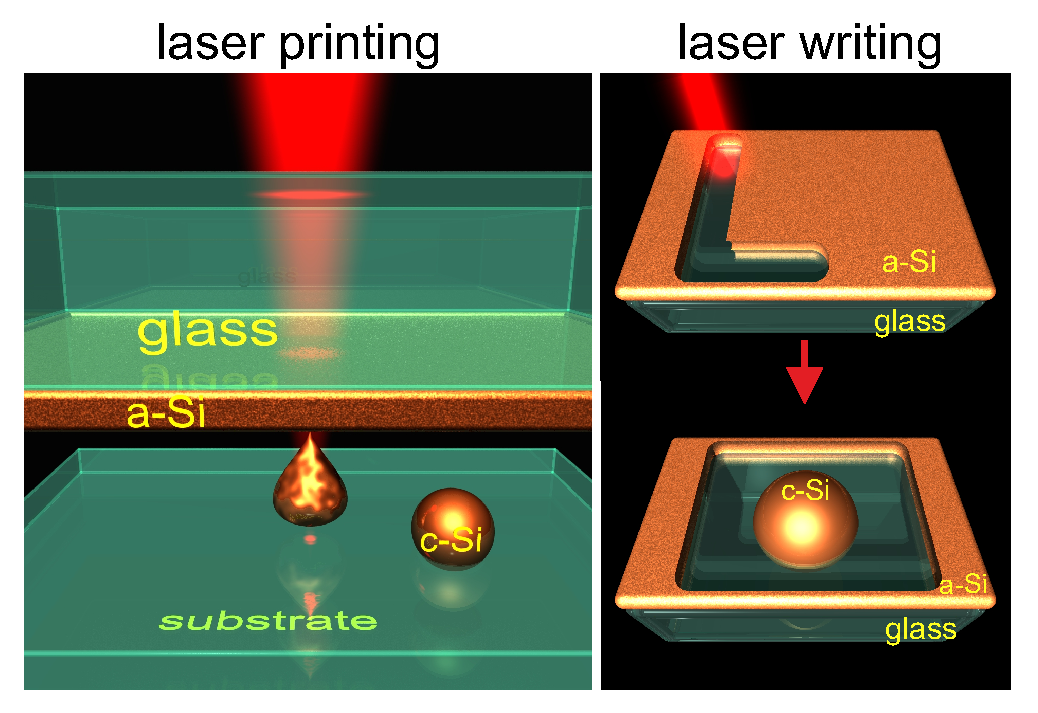
\includegraphics[width=0.5\textwidth]{figs/methods/LaserPrinting.eps}
                \end{center}
                \caption{Geometry of laser-ablation based fabrication methods of crystalline nanoparticles from amorphous
                            thin films.}
                \label{fig:LaserPrinting}
        \end{figure}

        \subsubsection{Laser Writing of Dielectric Particles}
        \label{met:writing}
                Laser writing of crystalline silicon nanoparticles was done directly in an initially amorphous thin film of a-Si:H.
            The film was patterned by a train of femtosecond pulses~--- by ablating the directly irradiated material, one can cut patches
            out of the a-Si film~\cite{makarov2016controllable},~\citeA{dmitriev2016direct}. The area irradiated by a single laser pulse
            with a fluence of $F\approx100~\si{mJ/cm^{2}}$ is brought close to the melting point of silicon, while using a pulse train with
            a delay of $12.5~\si{ns}$ between the pulses causes heat accumulation in the film, reaching and exceeding the ablation threshold.
                Heat is also transferred to the non-irradiated areas of the film, and tends to accumulate in the cut-out patches, because they
            are thermally isolated from the rest of the film, and the thermal conductivity of the substrate is much lower than the thermal
            conductivity of the film. Theses patches become unstable at high temperatures and can dewet to form a number of nanoparticles~\cite{thompson2012solid}.
            The size and number of the resulting nanoparticles can be controlled by laser fluence and repetition rate, cut patch size, and
            initial film thickness.

        \subsubsection{Laser Transfer of Crystalline Dielectric Particles}
        \label{met:transfer}

                Laser transfer of the nanoparticles was carried out using single femtosecond laser pulses. The particles were fabricated from
            a thin, amorphous, a-Si:H film in a forward transfer geometry (the relieving substrate is below the donor substrate and film, with a
            spacing of around $\sim 50~\si{\upmu m}$~--- see Fig.~\ref{fig:LaserPrinting}(a)). All of the particles were fabricated from
            previously undamaged areas of the silicon thin film. A forward-transfer geometry has an advantage over the back-transfer geometry
            that was presented in Ref.~\cite{zywietz2014laser}~--- it does not force the substrate to be transparent, allowing particles to be
            transferred to a wide variety of substrates, including structured, opaque samples.

                The single laser pulses required for the technique were selected from a train of femtosecond laser pulses by a Pockels cell
            pulse picker from Avesta Project. The pulses were focused by an $100\times$ Olympus oil immersion microscope objective with a
            numerical aperture of $\mathit{NA}=1.4$. Using the Rayleigh criterion, $\emph{d}\approx 1.22\lambda/\mathit{NA}$ the beam's focal
            spot size can be estimated to be $d=0.7~\si{\upmu m}$, which is closes to the value estimated by a method using the dependence
            of the area damaged by the laser on the laser energy ($0.68~\si{\upmu m}$)~\cite{liu1982simple}.

                The film used for the fabrication process was an $80~\si{nm}$ thick a-Si:H film deposited on afused silica substrate by
            plasma enhanced chemical vapor deposition (PECVD) from a SiH$_{3}$ precursor gas. Laser energies in the range of $0.5-1.2~\si{nJ}$, were used in the fabrication process, providing fluencies in
            the range of $0.12-0.16~\si{J/cm^{2}}$. The fabricated nanoparticles were to close being spherical in shape(figure~\ref{fig:Crystallinity}(b))
            and with diameters in the range of $50-200~\si{nm}$, depending on the fluence.

    \clearpage
    \subsection{Optical Measurements}
            All of the optical characterization measurements were carried out on a multifunctional setup, depicted in
            Fig.~\ref{fig:expSetup}. The setup allowed us to measure optical signals from single nanoparticles, provided that
            there was at least $1\mu$ m between the nanoparticle and its nearest neighbors. The XYZ-stage used for the
            positioning of the particles had $100$nm precision, giving enough control to position a single nanoparticle into
            the center of the excitation beam.

            The scattered light was collected from the top by an objective (Mitutoyo M Plan APO NIR, 100x, NA=0.7),
            sent to a Horiba LabRam HR spectrometer and projected onto a thermoelectrically cooled charge-coupled device
            (CCD, Andor DU 420A--OE 325) with a 150-g/mm diffraction grating. The spectrometer gave us a spectral resolution
            of around $1$nm.

            \begin{figure}[!ht]
                    \begin{center}
                        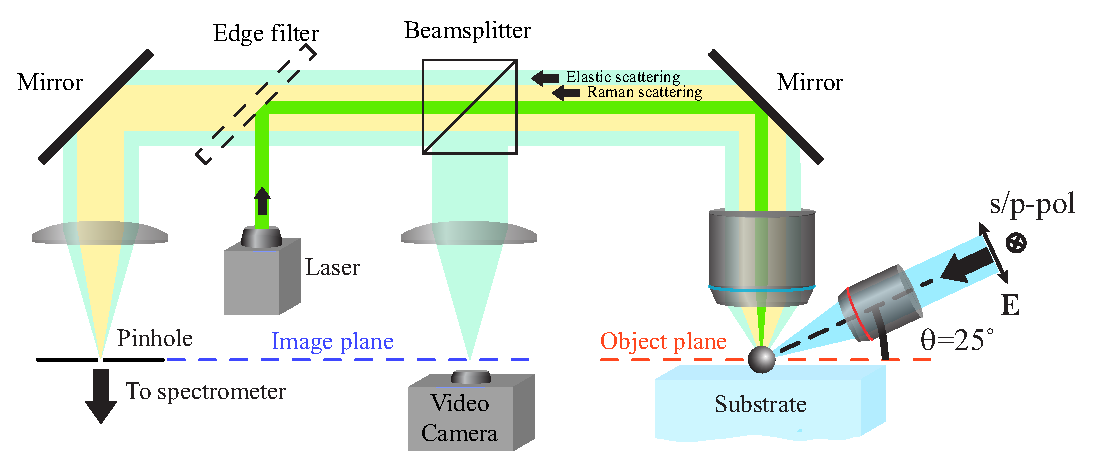
\includegraphics[width=0.9\textwidth]{figs/methods/expSetup2.eps}
                    \end{center}
                    \caption{Schematic of the experimental setup used for all of the optical measurements.}
                    \label{fig:expSetup}
            \end{figure}

        \subsubsection{Polarization-Resolved Dark-field Spectroscopy of Single Nanoparticles}
            \label{sec:Darkfield}
                For the dark-field scattering experiments, the nanoparticles were excited at an oblique angle of incidence
            (65 degrees to the surface normal) by linearly polarized light from a halogen lamp (HL--2000--FHSA)
            through a weakly-focusing objective (Mitutoyo M Plan Apo NIR, 10x, NA=0.28). The polarization allowed us to
            selectively excite different modes in the nanoparticles~\cite{permyakov2015probing}, see Fig.~\ref{fig:PolarizedDF}.

            \begin{figure}[!ht]
                    \begin{center}
                        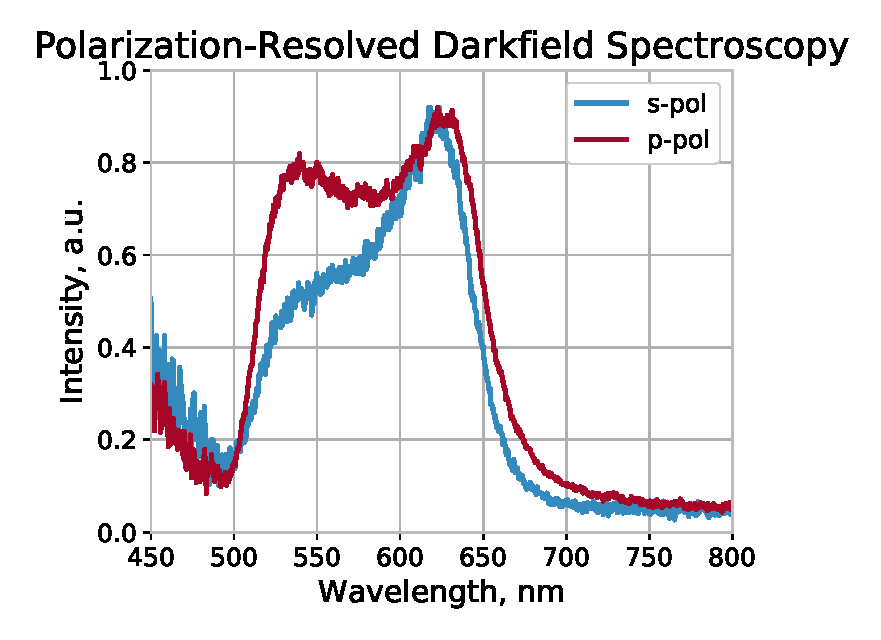
\includegraphics[width=0.6\textwidth]{figs/methods/DF/id_52780.eps}
                    \end{center}
                    \caption{Different Mie-type resonances excited by different polarizations of incident light.}
                    \label{fig:PolarizedDF}
            \end{figure}

        \subsubsection{Raman Spectroscopy of Single Nanoparticles}
        \label{sec:Raman}
                For the Raman scattering experiments, the nanoparticles were excited by one of two laser sources: a $632.8$nm HeNe laser
            or a $532$nm Nd:YAG laser, through the same channel that was used to collect the scattered light. A lowpass filter was used
            to filter out the excitation wavelength and leave only the Stokes-shifted inelastically scattered light.

                Raman intensity is proportional to the volume of the Raman-active material. One of the goals of the project was to compare
            the intensity of Raman scattering by particles with different resonance positions, which meant comparing particles of different
            sizes. This meant that for any meaningful comparison, the Raman signal had to be normalized to the volume of the particles, allowing
            comparisons of intensity per volume to be made.

    \subsection{Analytical Model of Raman Signal Enhancement by Mie resonances of Nanoparticles}
        \label{sec:Theory}
            This derivation is taken from the derivation in Ref.~\citeA{dmitriev2016resonant}.

             The rigorous Green tensor approach was used to describe the role of the electric and magnetic Mie resonances
        in the enhancement of Raman scattering of a silicon nanoparticle. The theoretical approach is based on earlier related
        studies~\cite{canccado2014theory, murphy1983enhanced}.

        The first was was to determine the spatial distribution of the electric field $\mathbf{E}_{exc}(\mathbf{r})$ at the excitation frequency
        inside the nanoparticle from an external source. Assuming a spherical particle, in free space, with illumination by a plane wave,
        the normalized electric field inside the nanoparticle can be decomposed into a series of vector spherical harmonics~\cite{bohren1983absorption}:

        %
        \begin{align}
            \mathbf{E}_{exc}(\mathbf{r})=\sum\nolimits_{n=1}^\infty E_n \left(c_n\mathbf{M}_{o1n}^{(1)}(\mathbf{r}) -
            i{d_n}\mathbf{N}_{e1n}^{(1)}(\mathbf{r})\right) ,
            \label{eq1}
        \end{align}
        %
        where $c_n$ and $d_n$ are Mie coefficients, ${{\mathbf{M}}_{o1n}^{(1)}}$ and ${{\mathbf{N}}_{e1n}^{(1)}}$~---
        orthogonal vectorial spherical harmonics, and ${E_n} = {i^n}(2n + 1)/[n(n + 1)]$. The distribution of the excitation electric field
        at each point inside the nanoparticles defines the Raman polarization oscillating the Stokes-shifted frequency $\omega_S$:
        %
        \begin{align}
            {{\bf{P}}_s}\left( {\bf{r}} \right) = {\chi _s}\hat \alpha_j \left( {\bf{r}} \right){{\bf{E}}_{exc}}\left( {\bf{r}} \right),
            \label{eq2}
        \end{align}
        %
        where $\chi_s$ is the scalar Raman susceptibility, $\hat \alpha_j$ is the Raman polarizability tensor representing
        the threefold degenerate transverse optical (TO) phonon mode excitation~\cite{ralston1970spontaneous, peter2010fundamentals}.

        The induced Raman polarization, then produces an electromagnetic field at an observation point
        $\mathbf{r}_0$:
        \begin{align}
            \mathbf{E}_s(\mathbf{r}_0) = (\omega_s^2/c^2)\int\limits_V {{{\hat G}_s}\left( {{{\mathbf{r}}_0},{\mathbf{r}}} \right){{\mathbf{P}}_s}\left( {\mathbf{r}} \right){d^3}{\mathbf{r}}}
        \end{align}
        where ${\hat G_s}\left( {{{\mathbf{r}}_0},{\mathbf{r}}} \right)$ is the Green tensor at the Stokes-shifted frequency, accounting
        for the Si nanoparticle. The integration is carried out over $V$, the volume of the nanoparticle. Then, the resulting signal at
        $\mathbf{r}_0$ can be written as:
        %
        \begin{align} %Final collected signal
            S\left( {{{\mathbf{r}}_0}} \right)
                =  \sum\limits_j {\left \langle{{\mathbf{E}}_s^*\left( {{{\mathbf{r}}_0}} \right){{\mathbf{E}}_s}\left( {{{\mathbf{r}}_0}} \right)} \right\rangle}
                = \sum\limits_j {\frac{{\omega _s^4}}{{{c^4}}}\iint\limits_V {{d^3}{{\mathbf{r}}_1}{d^3}{{\mathbf{r}}_2}\left\langle {\hat G_s^*\left( {{{\mathbf{r}}_0},{{\mathbf{r}}_1}} \right){\mathbf{P}}_s^*\left( {{{\mathbf{r}}_1}} \right){{\hat G}_s}\left( {{{\mathbf{r}}_0},{{\mathbf{r}}_2}} \right){{\mathbf{P}}_s}\left( {{{\mathbf{r}}_2}} \right)} \right\rangle }}  \\
                = \sum\limits_j {\frac{{\omega _s^4}}{{{c^4}}}\iint\limits_V {{d^3}{{\mathbf{r}}_1}{d^3}{{\mathbf{r}}_2}\hat G_s^*\left( {{{\mathbf{r}}_0},{{\mathbf{r}}_1}} \right){\mathbf{E}}_{exc}^*\left( {{{\mathbf{r}}_1}} \right){{\hat G}_s}\left( {{{\mathbf{r}}_0},{{\mathbf{r}}_2}} \right){{\mathbf{E}}_{exc}}\left( {{{\mathbf{r}}_2}} \right)\chi _s^2\left\langle {\hat \alpha _j^*\left( {{{\mathbf{r}}_1}} \right) \otimes {{\hat \alpha }_j}\left( {{{\mathbf{r}}_2}} \right)} \right\rangle }},
            \label{eq4}
        \end{align}
        %
        the summation is performed over the three degenerate TO phonon modes of silicon. Raman scattering is a spontaneous process
        (unless we are in the stimulated Raman scattering regime), meaning that the induced polarization $\mathbf{P}_s$ is not coherent across
        the particle. To account for that, the averaging in Eq.~(\ref{eq4}) is carried out over all possible orientations of Raman
        polarization $\mathbf{P}_s$. Because the correlation length of Raman scattering in silicon, $L_c$, is much less than the nanoparticle diameter
        (for particles resonant in the visible and near-infrared spectral ranges), being on the order of tens of nanometers, the is is possible to
        approximate the correlation of the Raman by the Dirac delta function:

        \begin{align}
            \left\langle {\hat \alpha_j \left( {{{\mathbf{r}}_1}} \right) \otimes \hat \alpha_j \left( {{{\mathbf{r}}_2}} \right)} \right\rangle \sim \delta \left({{\mathbf{r}_1} - {\mathbf{r}_2}} \right)
        \end{align}

        This reduces Eq.~(\ref{eq4}) to
        %
        \begin{align}
            S\left( {{{\bf{r}}_0}} \right) = \frac{{\omega _s^4}}{{{c^4}}}\sum\limits_j {\int\limits_V {{d^3}{\bf{r}}{{\left| {{{\hat G}_s}\left(
            {{{\bf{r}}_0},{\bf{r}}} \right){{\hat \alpha }_j}{\chi _s}{{\bf{E}}_{exc}}\left( {\bf{r}} \right)} \right|}^2}} }
            \label{eq5}
        \end{align}
        %
        \begin{figure}[h!]
            \begin{center}
                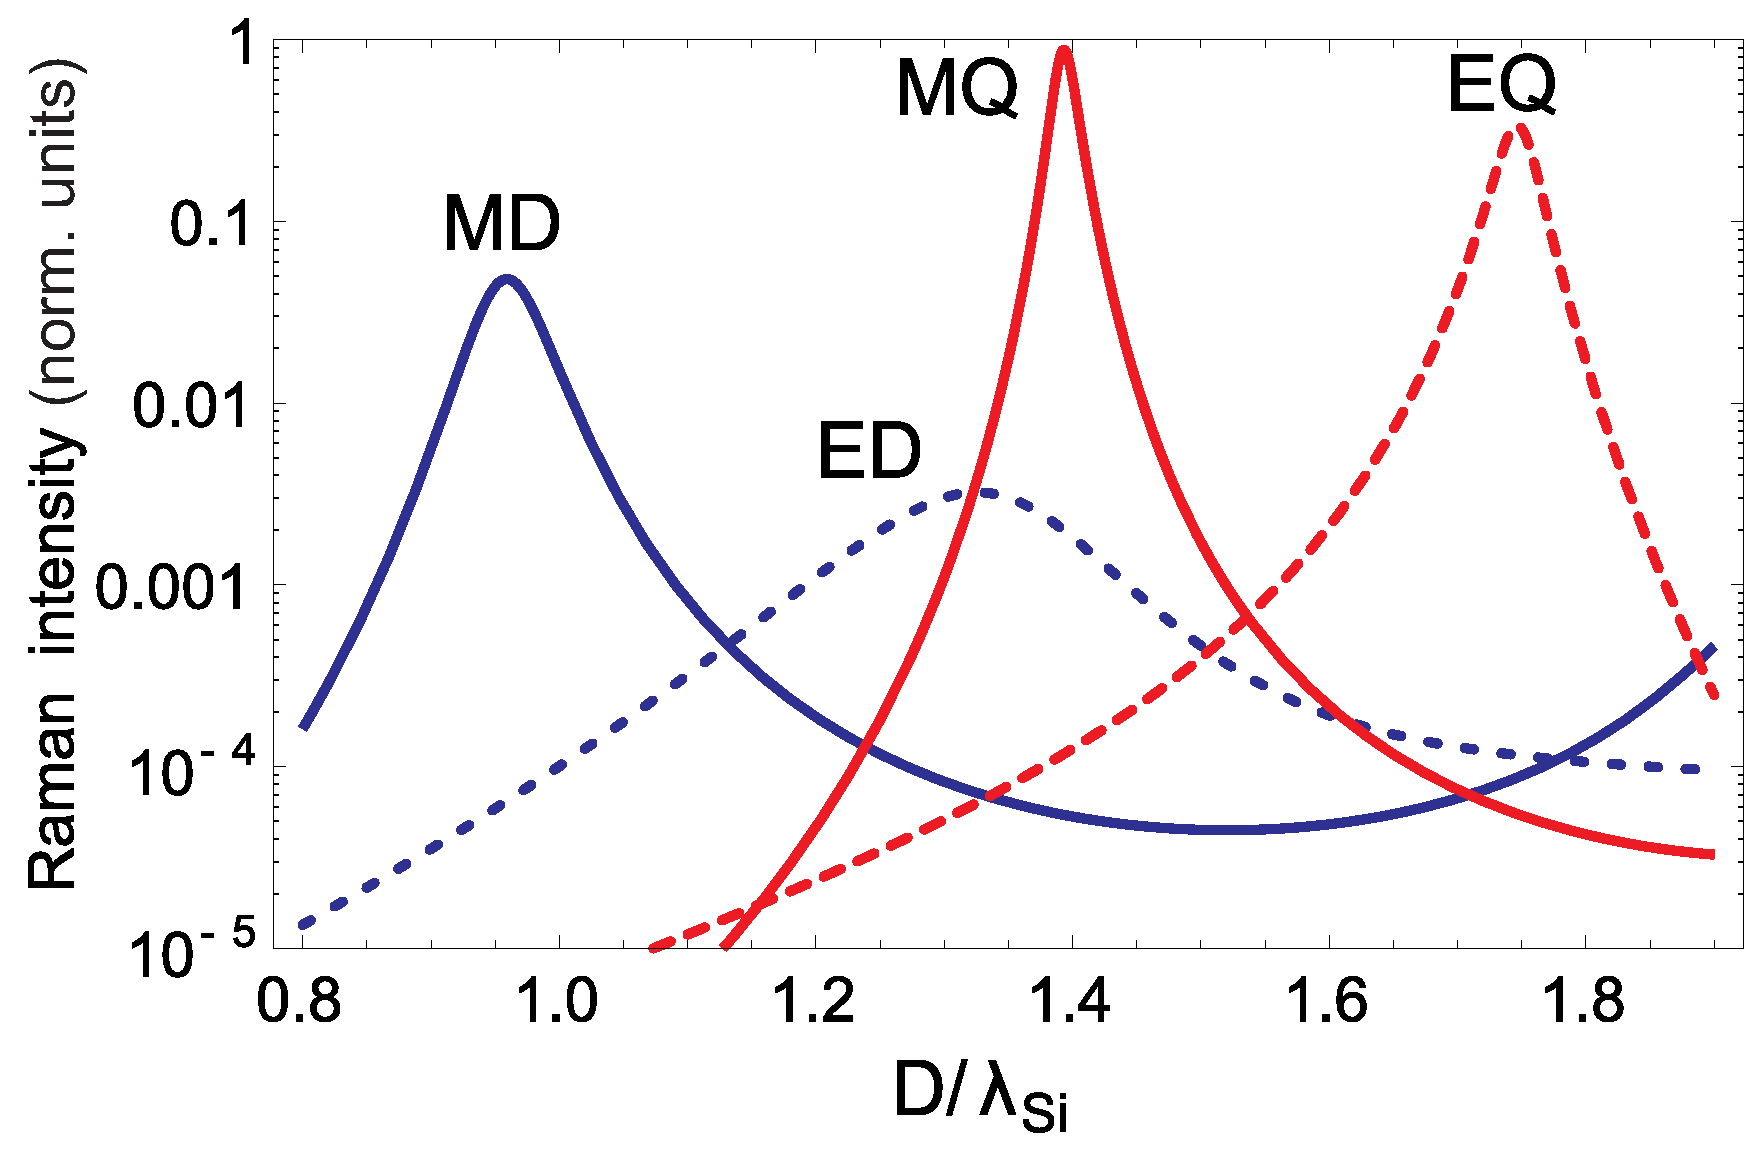
\includegraphics[width=0.5\textwidth]{figs/intro/TheoryEnhancement.eps}
            \end{center}
            \caption{Log plot of normalized intensity of Raman scattering as a function of dimensionless nanoparticle diameter for the magnetic dipole (MD),
            electric dipole (ED), magnetic quadrupole (MQ) and electric quadrupole (EQ) resonances.}
            \label{fig:TheoryEnhancement}
        \end{figure}

            Eq.~\ref{eq5} can be simplified by the single-mode approximation, which is applicable in this case, because the electromagnetic
        response of an optically small particle is always dominated by a single multipole resonance~\cite{evlyukhin2010optical}. Because
        of this, only one term from Eq.~\ref{eq1} is required to describe the electric field inside the nanoparticle:
        \begin{align}
            {{\mathbf{{E}}}_{exc}} \approx {E_n}{c_n}{\mathbf{M}}_{o1n}^{(1)} \\
            {{\mathbf{{E}}}_{exc}}\approx -i{E_n}{d_n}{\mathbf{N}}_{e1n}^{(1)}
        \end{align}
        For the $n-$th magnetic or $n-$th electric resonance.

        Because the Raman shift in silicon, compared to the linewidth $\gamma$ of Mie resonances at $\omega_0$, is small, the main contribution
        to the Green tensor is also provided by the same Mie resonance of the particle. Expanding the Green tensor in a series of
        eigenmodes~\cite{ishimaru1991electromagnetic} and discarding all therms except the resonant one:
        %
        \begin{align}
            {\hat G_s}\left( {{{\bf{r}}_0},{\bf{r}}} \right) \approx \frac{{{c^2}}}{{{N^2}}}\frac{{{\bf{u}}\left( {{{\bf{r}}_0}} \right) \otimes
            {\bf{u}}^*\left( {\bf{r}} \right)}}{{{{\left( {{\omega _0} + i\gamma } \right)}^2} - \omega _s^2}},
            \label{eq8}
        \end{align}
        %
        where ${{\mathbf{u}}\left( {{\mathbf r}} \right)}$ is the spatial distribution of the field of the eigenmode,
        ${N^2} = {\int {{\mathop{\rm Re}\nolimits} \varepsilon \left( {\bf{r}} \right)\left| {{\bf{u}}\left( {\bf{r}} \right)} \right|} ^2}{d^3}{\bf{r}}$
        is a normalization constant. After integrating Eq.~\ref{eq8} over the volume $V$ of the nanoparticle,
        an expression for Raman signal enhanced by a single Mie resonance, can be written:
        %
        \begin{align}
            S\left( {{{\mathbf{r}}_0}} \right) \approx V{\left( {\frac{{{\omega _s}}}{c}} \right)^4}{\left| {\frac{{{\chi_s s_n}}}{{{{\left( {{\omega
            _0} + i\gamma } \right)}^2} - \omega _s^2}}} \right|^2},
            \label{eq9}
        \end{align}
        %
        where $s_n$ stands for the Mie coefficient~--- either $c_n$ or $d_n$, electric or magnetic, of the mode. The equation
        shows that enhancement of Raman scattering depends on two main factors: enhancement of the excitation field
        inside the medium, and the Purcell enhancement of the Raman dipole radiation~\cite{checoury2010deterministic}.
        %
        Two main parameters in Eq.~(\ref{eq9}) are resonance frequency $\omega_0$ and linewidth $\gamma$. The first can be
        easily estimated numerically, and the second can be estimated by an analytical expression from Ref.~\cite{lai1991effect}.
        Using these values, The spectrum of Raman enhancement by different resonances of a spherical silicon nanoparticle can be plotted.
        Assuming a constant excitation wavelength of 633~nm (used in the Raman scattering experiments in this thesis), which corresponds to
        to a wavelength of $\lambda_{\rm Si}=163$~nm inside the nanoparticle, the spectrum, normalized to particle volume $V=4\pi R^3/3$, is
        plotted in Fig.~\ref{fig:TheoryEnhancement} as a  function of dimensionless nanoparticle diameter $D/\lambda_{\rm Si}$. The spectrum
        shows the contributions of the magnetic dipole (MD), electric dipole (ED), magnetic quadrupole (MQ) and electric quadrupole (EQ) resonances.

        Eq.~\ref{eq9}, being a single-mode expression, can be used to easily decompose the total Raman scattering enhancement into the constituent
        Mie resonance components. Fig.~\ref{fig:TheoryEnhancement} clearly shows, that the strongest enhancement is caused by the magnetic quadrupole
        resonance (MQ), owing to its high $Q-factor$. Another interesting fact is that the strongest Raman enhancement is caused by magnetic resonances,
        with both magnetic quadrupole (MQ) and dipole (MD) resonances out-performing their electric counterparts, EQ and ED, with MD being more than an
        order stronger than ED.

    \subsubsection{Numerical Methods}
    \label{sec:Numeric}
        Several numerical methods were used to simulate the scattering properties of the fabricated nanoparticles~--- to prove their
        crystalline phase, to probe their shape, to determine their size. The initial idea was to use the Discrete Dipole Approximation,
        because it is very flexible and can work with scatterers of arbitrary geometry. The main problem that was encountered was the fact
        the method is very involved (especially if one tries to incorporate substrate interaction), and computationally intensive for
        the required problems. Many calculations turned out to be excessive~-- a simple Mie theory calculation,
        while simulating a slightly different geometry, was more than enough to model the required parameters, with error well within the
        requirements.

        For calculations of field distribution inside the nanoparticles presented in this thesis, CST Microwave Studio was used.
        It is an  EM simulation package that uses the Finite Integration Technique for most of its calculations.

        \clearpage
        \subsubsection{Discrete Dipole Approximation}
        \label{subsec:DDA}

                For the DDA calculations, a custom, Python-based implementation was written, PyDDA~--- a reimplementation of an existing
            Matlab toolkit, DDA-SI~\cite{loke2011discrete}. The implementation even included surface-interaction components in its' calculations,
            but the complexity of the calculation and difficulty of accurately modeling particles led to the DDA being abandoned in favor of plain
            Mie theory, which provided more than enough accuracy for the purposes of the project.

            \begin{figure}[!ht]
                \centering
                \begin{subfigure}[b]{0.3\textwidth}
                    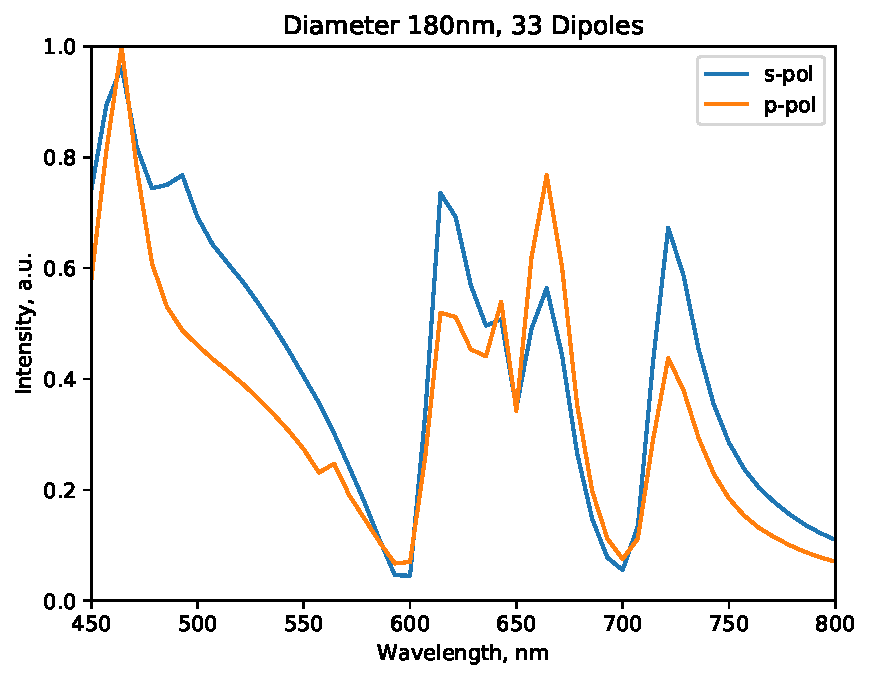
\includegraphics[width=\textwidth]{figs/methods/DDA/n_33.pdf}
                    \caption{}
                \end{subfigure}~
                \begin{subfigure}[b]{0.3\textwidth}
                    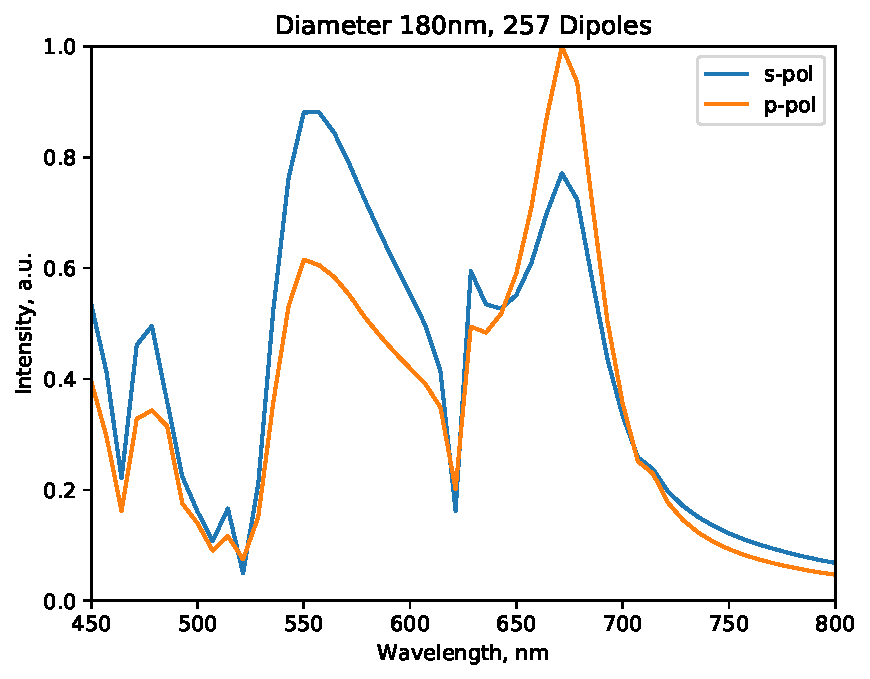
\includegraphics[width=\textwidth]{figs/methods/DDA/n_257.pdf}
                    \caption{}
                \end{subfigure}~
                \begin{subfigure}[b]{0.3\textwidth}
                    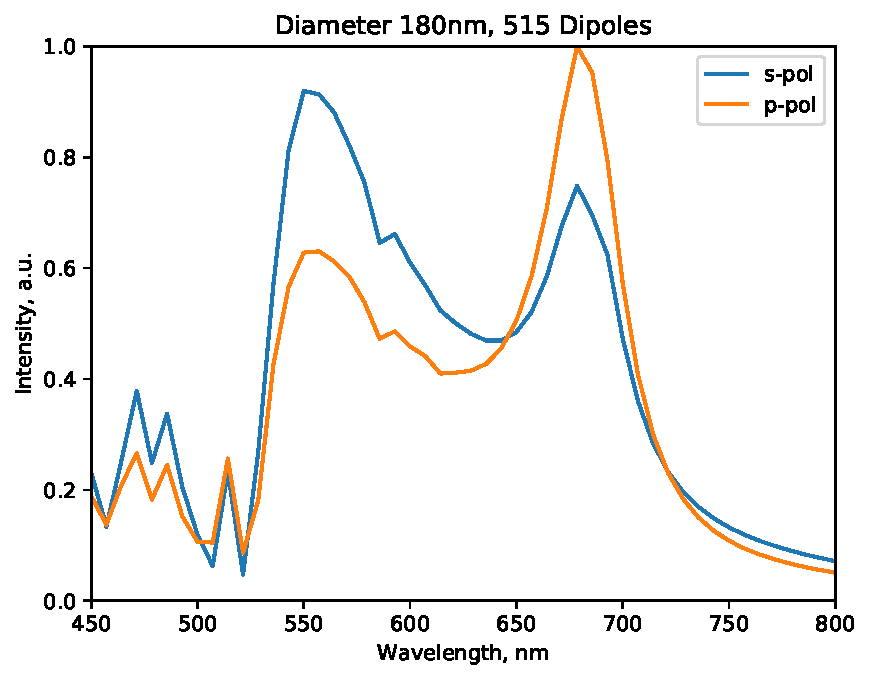
\includegraphics[width=\textwidth]{figs/methods/DDA/n_515.pdf}
                    \caption{}
                \end{subfigure}
                \caption{Scattering from isotropic sphere modeled by DDA using a) 33, b) 257, c) 515 dipoles to model the sphere.}
                \label{fig:DDA_Dipole}
            \end{figure}

        \subsubsection{Finite Integration Technique}
        \label{subsec:FIT}

                CST Microwave studio was used to model field distribution inside and around the silicon nanoparticles, to
            demonstrate the electric field confinement at different types of resonances (electric and magnetic dipole resonances).
            The model was a slightly oblate spheroid, corresponding to the experimentally determined geometric parameters of the
            nanoparticles.

            \begin{figure}[!hb]
                \centering
                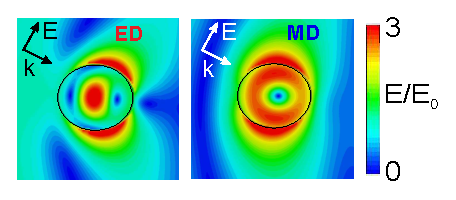
\includegraphics[width=0.7\textwidth]{figs/methods/FIT/CST.eps}
                \caption{Field distribution inside 180nm spheroid nanoparticle with 1.12 oblateness parameter at electric and magnetic dipole resonances,
                    calculated using CST Microwave Studio}
                \label{fig:CST}
            \end{figure}

\clearpage
